\subsection{Models already considered in Run-1}
Final states with two same-sign leptons and multiple jets are sensitive to a variety of new physics scenarios. 
In supersymmetric models in particular, such final states can be produced in the decays of heavy superpartners 
involving massive gauge bosons, sleptons or top quarks. 
We list in this section the different simplified models which we use as benchmarks for the choice of signal regions. 


\begin{figure}[h!]
\centering
\subfigure{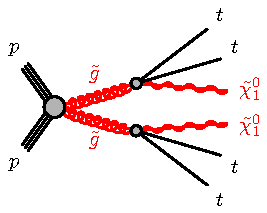
\includegraphics[width=0.24\textwidth]{MODELS/gogo-ttttN1N1}}
\subfigure{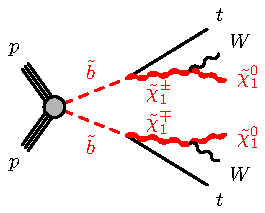
\includegraphics[width=0.24\textwidth]{MODELS/sbsb-ttWWN1N1}}
\caption{Gluino decay via offshell stop (left), and direct sbottom pair production (right).}
\label{fig:feynman_3rdgen}
\end{figure}

\begin{figure}[t]
\centering
\subfigure{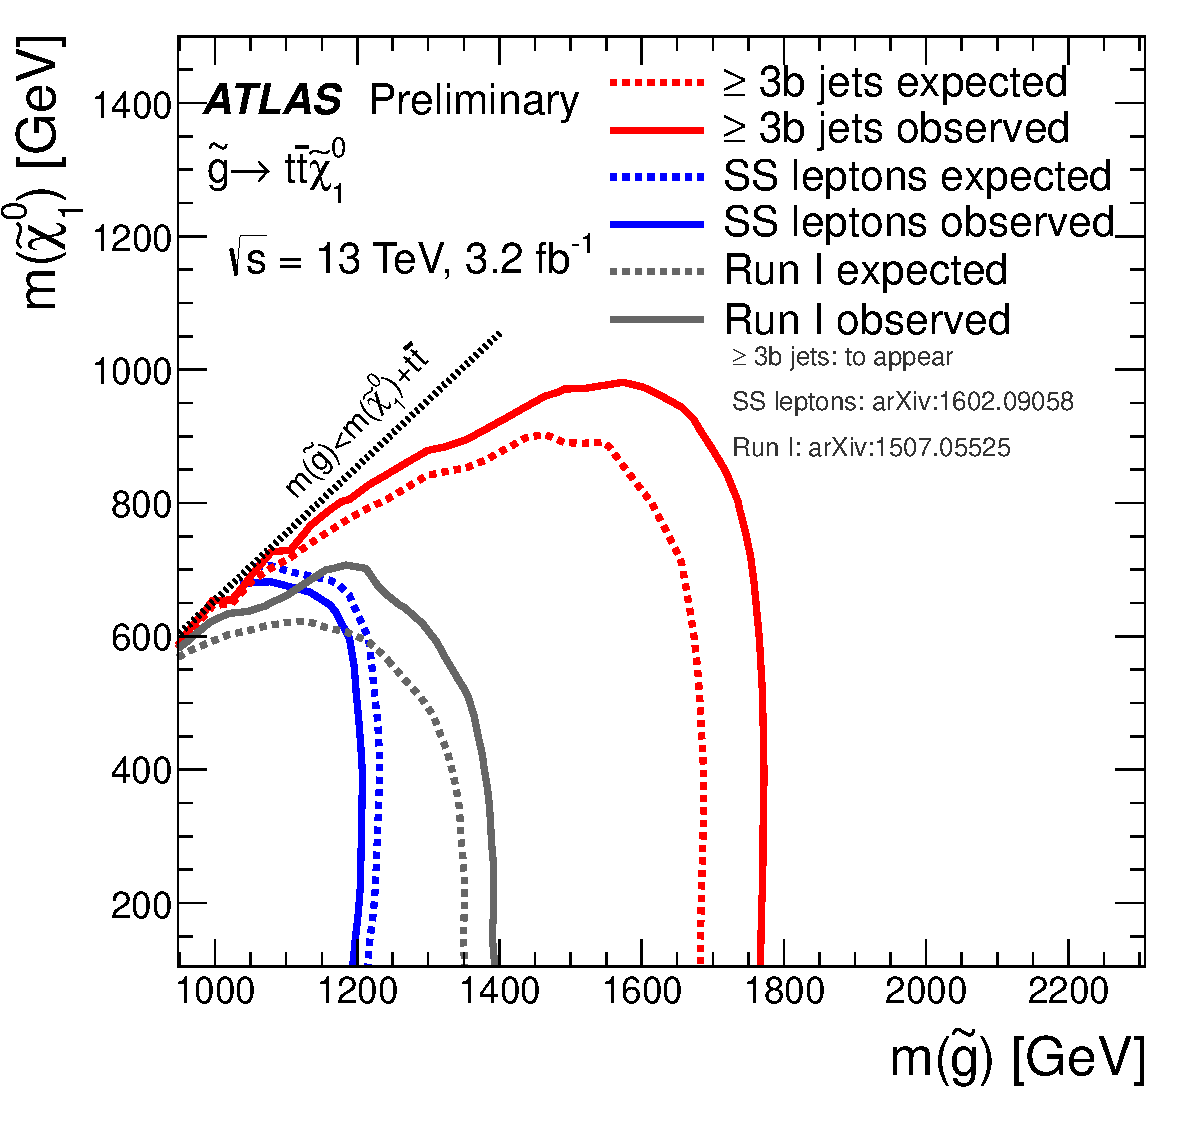
\includegraphics[width=0.49\textwidth]{MODELS/ATLAS_SUSY_Gtt}}
\subfigure{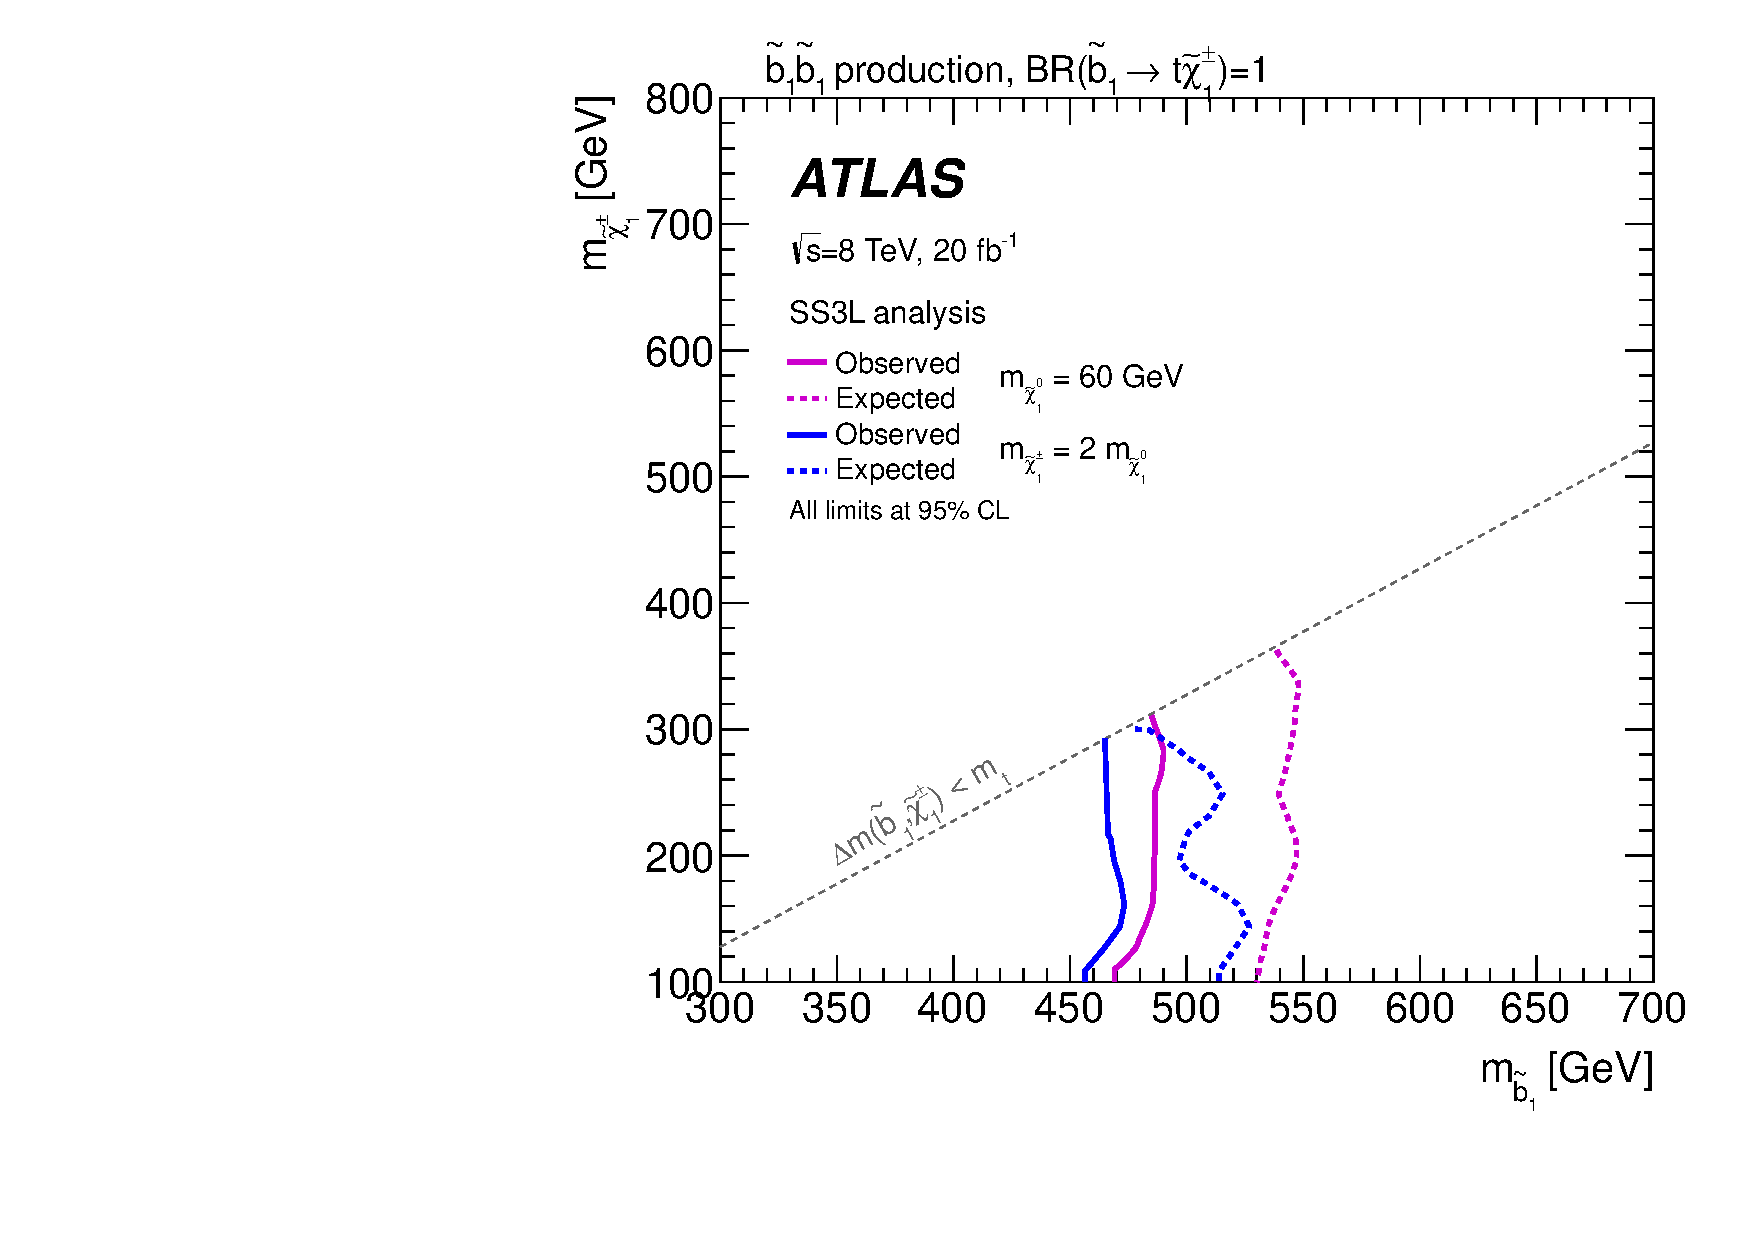
\includegraphics[width=0.49\textwidth]{MODELS/exclusion_sbottom_topC1_both_grids}}
\caption{Exclusion limits on the gluino-stop offshell (left) and direct sbottom (right) scenarios 
set by ATLAS with the 2012 dataset~\cite{DraftSquarkGluinoSummaryPaper}.}
\label{fig:run1excl_3rdgen}
\end{figure}

\par{\bf Gluino-stop offshell $\gluino\to t\bar t\neut$\\}
In this model inspired by naturalness arguments, gluinos are coupling preferentially to stops which are lighter than the other squarks. 
Gluinos are however considered lighter than stops, and decay directly into a $t\bar t\neut$ triplet via a virtual stop (Fig.~\ref{fig:feynman_3rdgen}). 
The pair production of gluinos leads to a final state containing four top quarks and two neutralinos. 
This characteristic final state is accessible through various experimental signatures, which is why this model 
is commonly used as a benchmark to estimate analyses sensitivities. 
The searches performed with run-1 data~\cite{DraftSquarkGluinoSummaryPaper}, 
summarized in Fig.~\ref{fig:run1excl_3rdgen}, showed that the same-sign leptons final state is competitive mainly at large neutralino mass. 
This region of the phase space is consequently given a particular attention in the choice of signal regions described further on. 
In the signal samples referenced in this document, the lightest stop mass is fixed to 10~\TeV and is mostly a $\widetilde{t}_R$ state. 
Only gluino pair production is considered, followed by an exclusive decay in the aforementioned channel. 
\\
\par{\bf Direct sbottom $\sbot\to t\chargino$\\}
In this model, bottom squarks are rather lights and assumed to decay in a top quark and a chargino $\chargino$ (Fig.~\ref{fig:feynman_3rdgen}), 
providing complementarity to the mainstream search which focuses on the channel $\sbot\to b\neut$. 
The final state resulting from the production of a sbottom pair contains pairs of top quarks, of $W$ bosons and of neutralinos. 
While this final state may lead to various experimental signatures, 
the model was considered in run-1~\cite{DraftSquarkGluinoSummaryPaper} 
only by the same-sign leptons and jets search, leading to the exclusion limits presented in Fig.~\ref{fig:run1excl_3rdgen}. 
In the signal samples used by the analysis, the neutralino mass is fixed to 60~\GeV, and the chargino mass to 150~\GeV, while the sbottom mass is varied. 
Only pair production of the lightest sbottom is considered, followed by an exclusive decay in the aforementioned channel. \\


\begin{figure}[h!]
\subfigure{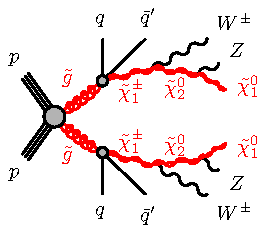
\includegraphics[width=0.24\textwidth]{MODELS/gogo-qqqqWWZZN1N1-C1N2}}
\subfigure{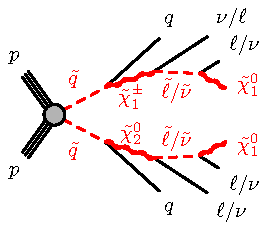
\includegraphics[width=0.24\textwidth]{MODELS/sqsq-qqlllvN1N1-C1N2}}
\subfigure{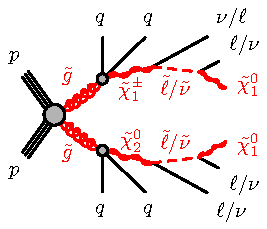
\includegraphics[width=0.24\textwidth]{MODELS/gogo-qqqqlllvN1N1-C1N2}}
\subfigure{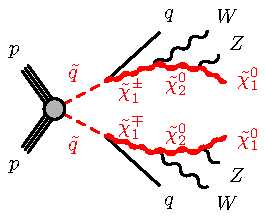
\includegraphics[width=0.24\textwidth]{MODELS/sqsq-qqWWZZN1N1-C1N2}}
\caption{Two-step decays of gluinos and squarks, mediated by gauginos (left) or sleptons (right).}
\label{fig:feynman_1stgen}
\end{figure}

\begin{figure}[t]
\centering
\subfigure{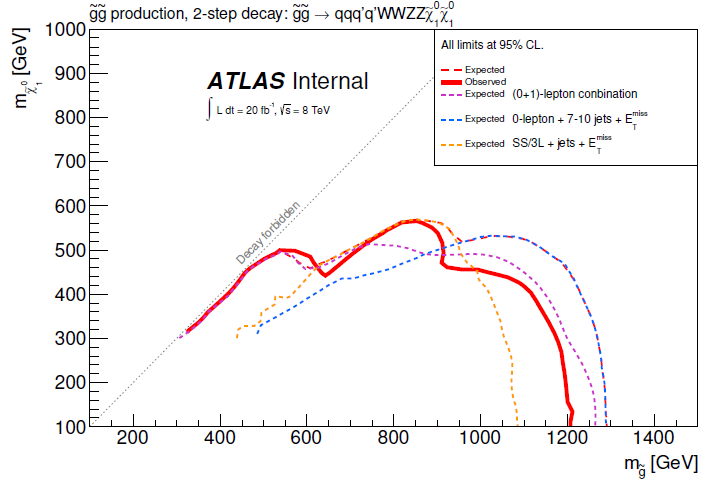
\includegraphics[width=0.49\textwidth]{MODELS/run1excluded_gluino2stepWZ}}
\subfigure{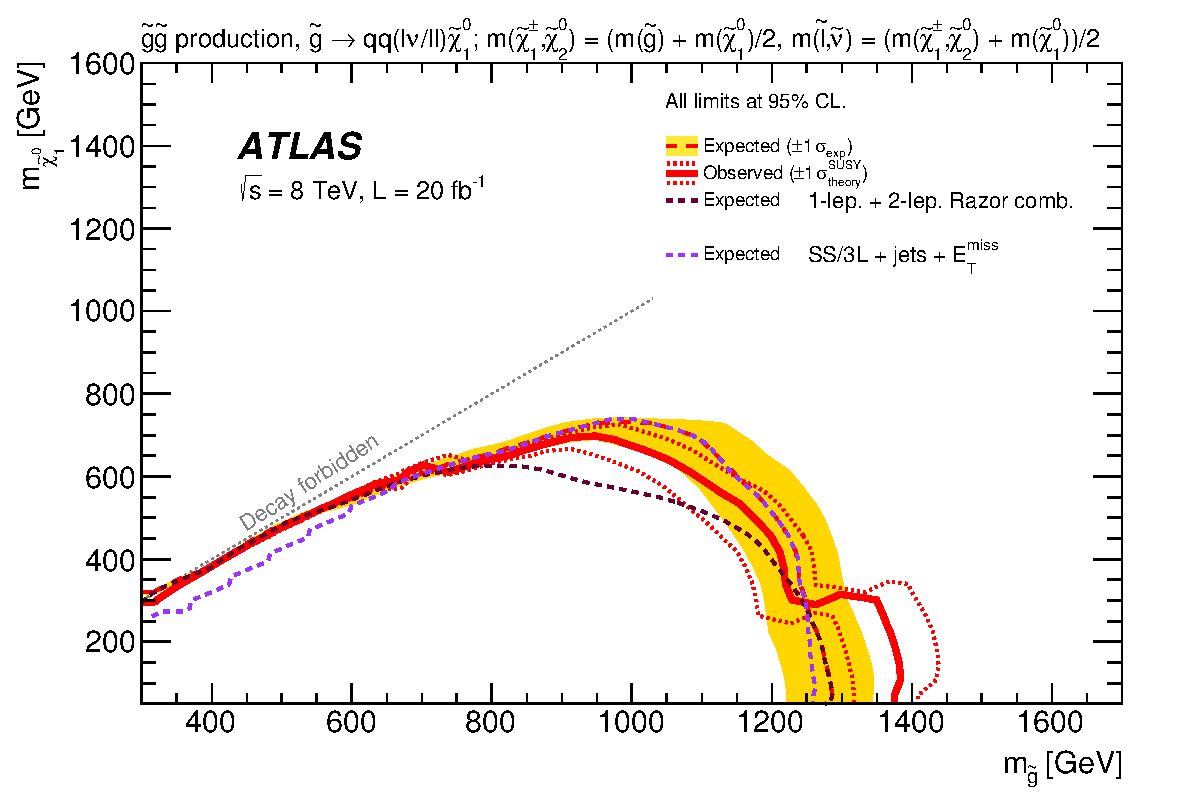
\includegraphics[width=0.49\textwidth]{MODELS/run1excluded_gluino2stepSleptons}}
\subfigure{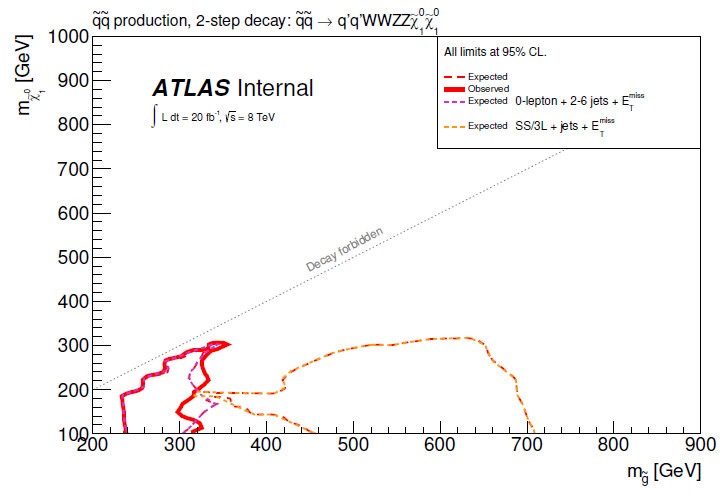
\includegraphics[width=0.49\textwidth]{MODELS/run1excluded_squark2stepWZ}}
\subfigure{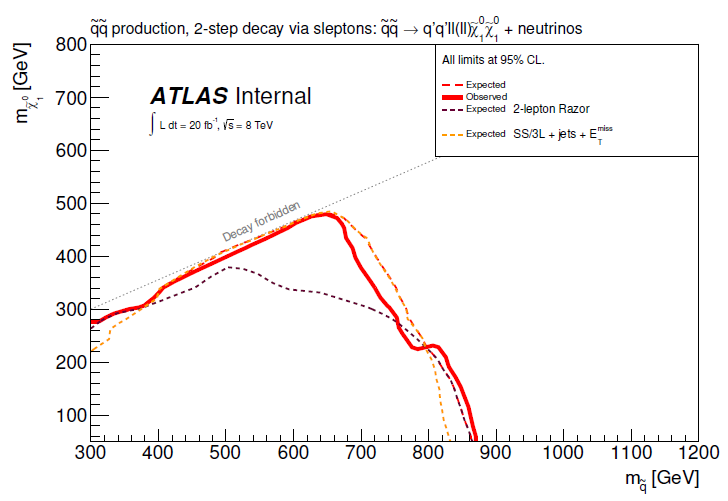
\includegraphics[width=0.49\textwidth]{MODELS/run1excluded_squark2stepSleptons}}
\caption{Exclusion limits on scenarios featuring gluino (top) and squarks (bottom) two-steps decays via gauginos (left) or sleptons (right) 
set by ATLAS with the 2012 dataset~\cite{DraftSquarkGluinoSummaryPaper}.}
\label{fig:run1excluded_1stgen}
\end{figure}

\par{\bf Gluinos and squarks 2-step decays via gauginos\\}
These scenarios feature a less oriented search for gluinos or squarks (save third generation) where gluinos couple preferentially to the latter, 
and squarks decay to charginos (Fig.~\ref{fig:feynman_1stgen} left) with the subsequent cascade $\chargino\to W\tilde{\chi}_{2}^{0} \to WZ\neut$. 
This leads to final states of two light quarks, two $W$ and $Z$ bosons, and two neutralinos 
(with two additional light quarks in the case of gluino pair production). 
Fig.~\ref{fig:run1excluded_1stgen} left shows the exclusion limits obtained with the 2012 dataset~\cite{DraftSquarkGluinoSummaryPaper}; 
in the gluino scenario, the same-sign leptons + jets search provided complementarity at large neutralino mass, 
while its sensitivity in the squark scenario dominated completely. 
In the signal samples used here, the chargino mass is set halfway between the neutralino and squark (or gluino) masses, 
while the neutralino $\tilde{\chi}_{2}^{0}$ mass is set halfway between the chargino and neutralino masses. 
Gluino and squark-antisquark pair production are considered separately in distinct scenarios.  
\\
\par{\bf Gluinos and squarks 2-step decays via sleptons\\}
In these scenarios, gluinos couple preferentially to the squarks of the first two generations, and
the latter decay either to a chargino $\chargino$ or a neutralino $\tilde{\chi}_{2}^{0}$, 
which are assumed to be mass-degenerate, and decay in turn to sleptons (Fig.~\ref{fig:feynman_1stgen} right) 
with $\mathcal{BR}(\chargino\to\nu\tilde\ell) = \mathcal{BR}(\chargino\to\ell\tilde\nu) 
= \mathcal{BR}(\tilde{\chi}_{2}^{0}\to\nu\tilde\nu) = \mathcal{BR}(\tilde{\chi}_{2}^{0}\to\ell\tilde\ell)=50\%$. 
The corresponding final state may contain zero to four charged leptons, neutrinos, two light quarks and two neutralinos 
(with two additional light quarks in the case of gluino pair production). 
Because of the sleptons replacing the gauge bosons featured in the scenarios presented in the previous paragraph, 
these scenarios have comparatively a lower jet multiplicity but a significantly enhanced acceptance in multi-lepton experimental signatures. 
As can be seen on Fig.~\ref{fig:run1excluded_1stgen} right, which presents the exclusion limits obtained with the 2012 dataset~\cite{DraftSquarkGluinoSummaryPaper}, 
the same-sign leptons and jets signature is again very competitive. 
In the signal samples used here, the chargino $\chargino$ and neutralino $\tilde{\chi}_{2}^{0}$ masses are set equal, 
halfway between the neutralino and squark (or gluino) masses, 
while the degenerate sleptons masses are set halfway between these gauginos and the lightest neutralino masses. 
Furthermore, gauginos decay to any slepton flavor with equal probability. 
Gluino and squark-antisquark pair production are considered separately in distinct scenarios. 
\\
\par{\bf Models not considered for the moment\\}
In the publications~\cite{paperSS3L,DraftSquarkGluinoSummaryPaper} of the analysis results obtained with run-1 data, 
exclusion limits were also provided for other signal models, often 
These scenarios included the $\gluino\to tbW\neut$ and $\gluino\to tcW\neut$ simplified models, as well as minimal models featuring 
$R$-parity violation through bilinear terms, gauge-mediated SUSY breaking, or universal extra dimensions. 
These models are not considered here, although interpretations might be proposed for them again in the future. 

\subsection{New models}

%\subsubsection{pMSSM inspired [Sebastien]}

\subsubsection{RPV inspired}
\label{subsec:RPVmodel}

 In supersymmetry, the following superpotential is present :
 \begin{align}
   W = \mu H L + \frac{1}{2} \lambda_{ijk} L_i L_j E_k + \lambda'_{ijk} L_i Q_j D_k + \frac{1}{2} \lambda''_{ijk} U_i D_j D_k
   \label{rpvpotential}
 \end{align}
 where $H$, $L$, $Q$, $E$, $U$ and $D$ are respectively the superpotential associated to the Higgs doublet, the lepton-neutrino doublet, the quark up-down doublet, the right-handed electron, the right-handed up quark and the right-handed down quark.
 The indices $i$, $j$ and $k$ are the flavor indices and $\mu$ , $\lambda_{ijk}$ , $\lambda'_{ijk}$ , $\lambda''_{ijk}$ are the coupling constants.
\\

 The leptonic number violation and the baryonic number violation implied by this potential have an important impact in the physic at low energy
 and do not respect some low energy constraints like the proton decay time limit.
 In $R$-parity conserving (RPC) SUSY models, the $R$-parity is added in order to remove these terms and keep the proton stable.
 However, one can play with the couplings $\mu$ , $\lambda_{ijk}$ , $\lambda'_{ijk}$ and $\lambda''_{ijk}$ in order to violate $R$-parity while respecting the low energy constraints.
 This is called the $R$-parity violation (RPV) SUSY models.
\\

 In this note, we will only consider the case where the coupling constants $\mu$, $\lambda_{ijk}$, $\lambda'_{ijk}$ and $\lambda''_{(i \neq 3) jk}$ are suppressed.
 Therefore, the only non-negligible terms are $\lambda''_{321}TSD$ , $\lambda''_{331}TBD$ and $\lambda''_{323}TSB$ where $T$, $B$, $D$ and $S$ are the superfields associated to the top, bottom, down and strange quark.
 This scenario is predicted by some RPV models like the Minimal Flavor Violation (MFV) scenarios~\cite{Nikolidakis:2007fc,Csaki:2011ge} and leads to the production of same-sign top quarks~\cite{Durieux:2013uqa} (see Fig.~\ref{fig:rpv_diagram}).

\begin{figure}[h!]
\centering
\subfigure{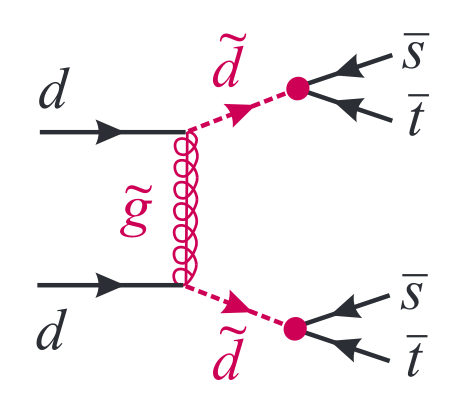
\includegraphics[width=0.24\textwidth]{MODELS/ddfusion.png}}
\subfigure{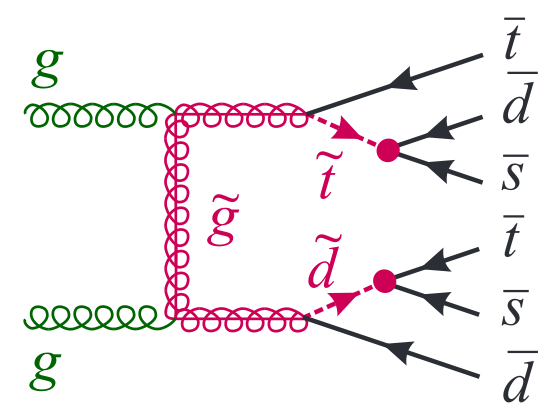
\includegraphics[width=0.27\textwidth]{MODELS/ggfusion.png}}
\caption{Example of diagrams for RPV model for the \textit{d-quark fusion} topology (left), and the \textit{gluon fusion} topology (right) involving the $\lambda''_{321}$ coupling. In both cases, the baryonic number is violated by two units. }
\label{fig:rpv_diagram}
\end{figure}

 In these scenarios, the $R$-parity is not conserved and the LSP is not stable (and therefore cannot be a good dark matter candidate).
 However, the interesting part of this model is that it allows B-violating processes (see Fig.~\ref{fig:rpv_diagram}).
 Actually, the baryonic asymmetry in the universe and the fact that the standard model does not respect this symmetry provides a good motivation for the search for $B$-violation processes at high energy.
 In addition, it was also proved that the violation of the baryonic number by two units involving top quarks could respect the low denergy constraints like the proton decay time limit~\cite{Durieux:2012gj}.
% Therefore, RPV SUSY is good generic model for the search for $B$-violation.
\\

In this analysis, two kind of topologies will be considered:
\begin{itemize}
\item \textbf{d-quark fusion}: Production of two on-shell $d$-squarks with a gluino in $t$-channel and the $d$-squarks decay to an anti-top quark and to one extra jet.
  The squarks will lighter than the gluino and the cross section will mostly depend on the mass of the squark (see Fig.~\ref{fig:rpv_diagram}).
  \begin{align}
    dd \to \tilde{d} \tilde{d}\ ,\ \tilde{d} \to \bar{t}q    
  \end{align}
\item \textbf{gluon fusion}: Production of two on-shell gluinos which decay to a top or an anti-top quark and to two extra jets.
  The gluino will be lighter than the squarks and the cross section will only depend on the mass of the gluino (see Fig.~\ref{fig:rpv_diagram} ).
  \begin{align}
    gg \to \gluino\gluino\ ,\ \gluino \to tqq\ /\ \gluino \to \bar{t}qq'
  \end{align}
\end{itemize}
The extra jets could be either $b$-jet or light jets, depending on the coupling being considered. 
In order to have access to the charge of the top quark, we will only consider the case where the top quark decays leptonically.
At the end, the final states will be composed of two same-sign leptons, at least two $b$-jets, low missing transverse energy (coming from the neutrinos) and extra jets.
\\
% Cross section : soon

 This model was already constrained by ATLAS~\cite{Aad:2014pda} and CMS~\cite{Chatrchyan:2013fea} in Run-1, but those analyses 
 only considered the coupling $\lambda''_{323}$ and the topology of \textit{gluon fusion}.
 A limit of around 900 GeV was found on the mass of the gluino. The full hadronic final state was also exploited in ATLAS~\cite{Aad:2013wta}.

